\documentclass[conference]{IEEEtran}
\usepackage[table]{xcolor}
\usepackage{tabularx}
\usepackage{graphicx}
\usepackage{amsmath}
\usepackage{listings}
\lstset{basicstyle=\ttfamily, frame=single, language=python, tabsize=4}
\usepackage{tikz}
\usetikzlibrary{arrows.meta, automata, quotes, positioning, babel, shapes.geometric, arrows}
\usepackage{booktabs}

\begin{document}
\title{Node embedding analysis with Model R}
\author{
	\IEEEauthorblockN{name}
	\IEEEauthorblockA{
		address1 \\
		address2 \\
		email
	}
	\and
	\IEEEauthorblockN{name}
	\IEEEauthorblockA{
		address1 \\
		address2 \\
		email
	}
}
\maketitle

\begin{abstract}
Deep learning models based on node embedding techniques are becoming increasingly successful in graph mining tasks such as predicting node and link attributes.
The main reason for their success is based on the assumption of their ability to extract knowledge of nodes (i.e., node embeddings) from the relations between nodes (i.e., links).
However, there are few studies or evidences to justify this assumption.
Here we present an in-depth node embedding analysis with Model R - a recent node embedding based deep learning model.
This work provides strong evidences that Model R indeed has the ability to extract knowledge of nodes from the relations between nodes.
\end{abstract}
	
\section{Introduction}
Embeddings are ubiquitous in deep learning, appearing in natural language processing, recommender systems, graph mining and other applications.
Embeddings refer to vectors of numbers representing entities such as
words (in natural language processing),
items (in recommender systems) and
nodes (in graph mining).
Embedding also refers to
the process of converting entities to points in an embedding space,
or equivalently,
the process of mapping entities to vectors in a vector space.
Recent embedding techniques either use the skip-gram model, such as
word2vec \cite{mikolov2013linguistic},
doc2vec \cite{le2014distributed},
item2vec \cite{barkan2016item2vec},
node2vec \cite{grover2016node2vec} and
deep walk \cite{perozzi2014deepwalk},
or use model R \cite{hou2017deep}.
All these techniques have achieved high prediction accuracies in their various applications including language modeling, item rating prediction, node classification and link weight prediction.
There are substantial studies in word embedding analysis with Skip-gram model \cite{mikolov2013distributed}.
These studies provide strong evidence that word embedding with the skip-gram model can extract knowledge about words from the relations between words and represent this knowledge in the word embedding space.
However, there are few studies related to node embedding analysis.

The contribution of this paper is that it provides strong evidence that node embedding with Model R can extract knowledge about nodes from the relations between nodes and represent this knowledge in the node embedding space.
This work also provides a potential approach to recommender systems based on node embeddings that recommends closest items to an item a customer recently purchased or liked.
We follow the approach used for word embedding analysis with the skip-gram model in our analysis on node embedding analysis with Model R(as well as item embedding, which is a special case of node embedding where the graph is a bipartite graph).

\section{Entity embedding techniques}
In this section, we review a few classical embedding techniques and models for images, audio, words, documents, items and nodes.
A common goal of these techniques is to ensure that
similar entities are close to each other in the embedding space.

\subsection{Content-based embedding techniques}
Techniques in this group extract knowledge about an entity from its content, 
i.e., the input of the neural network is a vector produced from the item's content.
For example, the content can be the pixel values of an image, or the spectrogram of an utterance.
The similarity of these techniques is that the content (the raw input to the neural network) is already a vector.
Therefore, the embedding process is practically a dimensionality reduction process
that converts a high dimensional raw input vector to a low dimensional vector 
containing more abstract knowledge about the input entity.

\subsubsection{Image embedding with auto-encoders}
This is an unsupervised embedding technique commonly used in feature learning
or representation learning \cite{liou2008modeling}.
A small auto-encoder neural network model is shown
in Figure \ref{fig:audoEncoder}.
\begin{figure}[!ht]	
	\centering
	\newcommand{\layersep}{2cm}
	\newcommand{\vocabularySize}{8}
	\begin{tikzpicture}
	[->, shorten >=1pt,node distance=\layersep]
	\tikzstyle{every pin edge}=[shorten <=1pt]
	\tikzstyle{neuron}=[circle, draw=black, minimum size=16pt, fill=green!30]
	
	\foreach \name / \y in {1,...,\vocabularySize}
	\node(input-\name) [neuron, fill=red!30, pin={[pin edge={<-}]below:}] at (\y, 0) {};	
	\node [below of=input-4, xshift = 0.5cm, yshift = 1cm] {input = the image pixel values};
	
	\foreach \name / \y in {1,...,4}
	\path[xshift=2cm]
	node(hidden1-\name) [neuron] at (\y, 1*\layersep) {};
	
	\foreach \name / \y in {1,...,2}
	\path[xshift=3cm]
	node(hidden2-\name) [neuron] at (\y, 2*\layersep) {};	
	\node [right of=hidden2-2] {embedding layer};
	
	\foreach \name / \y in {1,...,4}
	\path[xshift=2cm]
	node(hidden3-\name) [neuron] at (\y, 3*\layersep) {};
	
	\foreach \name / \y in {1,...,\vocabularySize}
	\node(output-\name) [neuron, fill=blue!30, pin={[pin edge={->}]above:}] at(\y, 4*\layersep) {};
	\node [above of=output-4, xshift = 0.5cm, yshift = -1cm] {output = the image pixel values};
	
	\foreach \source in {1,...,\vocabularySize}
	\foreach \dest in {1,..., 4}
	\path (input-\source) edge (hidden1-\dest);
	
	\foreach \source in {1,...,4}
	\foreach \dest in {1,...,2}
	\path (hidden1-\source) edge (hidden2-\dest);
	
	\foreach \source in {1,...,2}
	\foreach \dest in {1,...,4}
	\path (hidden2-\source) edge (hidden3-\dest);
	
	\foreach \source in {1,...,4}
	\foreach \dest in {1,...,\vocabularySize}
	\path (hidden3-\source) edge (output-\dest);
	\end{tikzpicture}
	\caption{
		A small auto-encoder neural network model with
		1 input layer (red), 3 hidden layers (green), and 1 output layer (blue),	input size 8, embedding size 2.
		Notice that the embedding layer is the innermost hidden layer.
		The hidden layers use rectified linear units.
		The output layer uses linear units.
	}
	\label{fig:audoEncoder}
\end{figure}
The model is a feed-forward neural network.
The output layer and the input layer have the same size.
The hidden layers closer to the input or output layers have larger sizes.
This technique is unique because during training,
the input activation and the expected output activation are always
the same vector of pixel values of the image.
From the input layer to the embedding layer, the layer size decreases,
compressing the information.
It can effectively reduce a high dimensional vector (the activation of a large number of input units with raw pixel values)
to a low dimensional vector (the activations of a small number of hidden units with abstracted meanings)
\cite{hinton2006reducing}.

\subsubsection{Audio embedding with convolutional neural network}
This is a supervised deep learning technique commonly used in audio classification.
A small convolutional neural network model is shown in Figure \ref{fig:cnn}.
\begin{figure}[!ht]
	\centering
	\newcommand{\layersep}{1cm}
	\begin{tikzpicture}
	[->, shorten >=1pt,node distance=\layersep]
	\tikzstyle{every pin edge}=[shorten <=1pt]
	\tikzstyle{layer} = [rectangle, text centered, draw=black, fill=green!30]
	
	\node (input) [layer, fill=red!30, pin={[pin edge={<-}]below:}] {direct activation layer};
	\node [below of=input] {input = the audio spectrogram};

	\node (hidden1) [layer, above of=input] {convolutional layer};
	\node (hidden2) [layer, above of=hidden1] {pooling layer};
	\node (hidden3) [layer, above of=hidden2] {convolutional layer};
	\node (hidden4) [layer, above of=hidden3] {pooling layer};
	\node (hidden5) [layer, above of=hidden4] {fully connected layer};
	\node [right of=hidden5, xshift = 2cm] {embedding layer};
	
	\node (output) [layer, fill=blue!30, above of=hidden5, pin={[pin edge={->}]above:}] {fully connected layer};
	\node [above of=output] {output = the target label};
	
	\path (input) edge (hidden1);
	\path (hidden1) edge (hidden2);
	\path (hidden2) edge (hidden3);
	\path (hidden3) edge (hidden4);
	\path (hidden4) edge (hidden5);
	\path (hidden5) edge (output);
	
	\end{tikzpicture}
	\caption{
		A small convolutional neural network model with
		1 input layer (red), 5 hidden layers (green), and 1 output layer (blue).
		Notice that the embedding layer is the last hidden layer.
		The hidden layers use rectified linear units.
		The output layer uses softmax units.
		Only layers and the connections between layers are shown, while the units in each layer and the connections between units are not shown.
	}
	\label{fig:cnn}
\end{figure}
The model is a feed-forward neural network.
The input layer is activated by
an image,
an audio spectrogram \cite{van2013deep} or
a letter tri-gram vector of a document \cite{elkahky2015multi}.
The output layer uses softmax units to predict the target label,
such as the genre, instrumentation of a song or the topic of an article.
From the input layer upward,
each convolutional and pooling layer combo extracts more abstract information
than the previous layer.
Eventually, the neural network converts the raw input data to an embedding
at the fully connected layer and uses it to predict the target label.
Most of the studies on convolutional neural networks focus on accurately
predicting the target attributes,
and the concept of entity embedding is under-explored.

\subsection{Relation-based embedding techniques}
Techniques in this group extract knowledge about an entity from its relations 
with other entities, such as words, users, items, and nodes.
The input of the neural network is the one-hot encoding vector of an entity.
An example of this encoding is shown in Table \ref{tab:one-hot}.
\begin{table}[!ht]
	\centering
	\caption{One hot encoding example for a dictionary of words.}
	\begin{tabular}{cc} \hline \rowcolor{blue!30}
		Word & One-hot encoding \\ \hline
		$ w_1 $ & [1, 0, 0, 0, ... 0]       \\ \hline
		$ w_2 $ & [0, 1, 0, 0, ... 0]       \\ \hline
		$ w_3 $ & [0, 0, 1, 0, ... 0]       \\ \hline
		$ w_4 $ & [0, 0, 0, 1, ... 0]       \\ \hline
		... & ...       \\ \hline
	\end{tabular}
	\label{tab:one-hot}
\end{table}
The similarity of these techniques is that each entity does not contain any
information about itself and therefore its one-hot encoding vector is also
a meaningless vector.
In other words, each entity is only defined by its relations with other entities.
Therefore, the embedding process is a process where the neural network gradually
forms understanding on the meanings of each entity by observing the relations
between all entities.
\subsubsection{Word embedding with skip-gram model}
This is an unsupervised embedding technique commonly used in
natural language processing \cite{mikolov2013linguistic}.
A small skip-gram neural network model is shown in Figure \ref{fig:skipGram}.
\begin{figure}[!ht]
	\centering
	\newcommand{\layersep}{2cm}
	\newcommand{\vocabularySize}{8}
	\newcommand{\embeddingSize}{4}
	\begin{tikzpicture}
	[->, shorten >=1pt,node distance=\layersep]
	\tikzstyle{every pin edge}=[shorten <=1pt]
	\tikzstyle{neuron}=[circle, draw=black, minimum size=16pt, fill=green!30]
	
	\foreach \name / \y in {1,...,\vocabularySize}
	\node[neuron, fill=red!30, pin={[pin edge={<-}]below:}] (input-\name) at (\y, 0) {};
	\node [below of=input-4, xshift = 0.5cm, yshift = 1cm] {input = word's one-hot encoding};
	
	\foreach \name / \y in {1,...,\embeddingSize}
	\path[xshift=2cm]
	node[neuron] (hidden-\name) at (\y, 1*\layersep) {};
	\node [right of=hidden-4] {embedding layer};
	
	\foreach \name / \y in {1,...,\vocabularySize}
	\node[neuron, fill=blue!30, pin={[pin edge={->}]above:}] (output-\name) at (\y, 2*\layersep) {};
	\node [above of=output-4, xshift = 0.5cm] {expected output = context-word's one-hot encoding};
	\node [above of=output-4, xshift = 0.5cm, yshift = -1cm] {actual output = context-word probability distribution};
	
	\foreach \source in {1,...,\vocabularySize}
	\foreach \dest in {1,...,\embeddingSize}
	\path (input-\source) edge (hidden-\dest);
	
	\foreach \source in {1,...,\embeddingSize}
	\foreach \dest in {1,...,\vocabularySize}
	\path (hidden-\source) edge (output-\dest);
	
	\end{tikzpicture}
	\caption{
		A small skip-gram neural network model with
		1 input layer (red), 1 hidden layer (green), and 1 output layer (blue),
		vocabulary size 8 and embedding size 4.
		Notice that the embedding layer is the hidden layer.
		The hidden layer uses linear units.
		The output layer uses softmax units.
	}
	\label{fig:skipGram}
\end{figure}
The model is a feed-forward neural network.
The definition of context is the set of words close to the middle word.
For example, given a natural language sentence:
\begin{align*}
	&sentence = [\\
	&the, quick, brown, fox, jumps, over, the, lazy, dog\\
	&]\\
\end{align*}
and a context radius:
\[context\_radius = 2\]
and a word:
\[word = fox\]
and the vocabulary:
\begin{align*}
	&vocabulary = [\\
	&the, quick, brown, fox, jumps, over, lazy, dog\\
	&]\\
\end{align*}
we have the context of [fox]:
\[ context(fox) = \{quick, brown, jumps, over\} \]
A natural language corpus has many sentences,
therefore, from these sentences we can produce a dataset where each example is a (word, context-word) pair,
as shown in Table \ref{tab:words}.
\begin{table}[!ht]
	\centering
	\caption{The words dataset for a natural language corpus.}
	\begin{tabular}{cc} \hline \rowcolor{blue!30}
		Input = word & Output = context-word \\ \hline
		... & ...       \\ \hline
		brown & fox \\ \hline
		brown & jumps \\ \hline
		fox & quick \\ \hline
		fox & brown \\ \hline
		fox & jumps \\ \hline
		fox & over \\ \hline
		jumps & brown \\ \hline
		jumps & fox \\ \hline
		... & ...       \\ \hline
	\end{tabular}
	\label{tab:words}
\end{table}
Given a word, its context word is a random variable with a probability distribution:
\[P(context\_word = x | middle\_word = fox)\]
where
\[x \in vocabulary\]
and the context-word probability distribution sums up to 1 over the vocabulary:
\begin{align*}
	&\sum_{x \in vocabulary}P(context\_word = x | middle\_word = fox)\\
	&= 1\\
\end{align*}
During each training step, one training example - a (word, context-word) pair - is used.
The input layer is activated by the one-hot encoding of the middle word.
The output layer is expected to predict the one-hot encoding of the context-word.
However, as each word can have many possible context-words, there is always a difference between the expected output and the actual output.
After substantial training, a skip-gram neural network model will eventually output the context-word probability distribution,
even though it is expected to output the one-hot encoding of the one context-word in the training example.
The embeddings for all words are technically the weights in the embedding layer.
For any natural language corpus and any two words X and Y in this corpus, we have the following equivalent statements:
\begin{itemize}
	\item X and Y have similar meanings
	\item X and Y have similar context-word possibility distribution 
	\item X and Y have similar embeddings
\end{itemize}
The final outcome is similar words have similar embeddings.
These embeddings are valuable in many natural language processing tasks.

\subsubsection{Item embedding with skip-gram model}
This is an embedding technique similar to word embedding, commonly used in recommender systems \cite{barkan2016item2vec}.
This technique reduces the item embedding problem to the word embedding problem and then applies the word embedding technique.
For example, given a purchase order:
\[ order = \{monitor, keyboard, mouse, printer, scanner\} \]
we have the context of [mouse]:
\[ context(mouse) = \{monitor, keyboard, printer, scanner\} \]
An e-commerce platform has many purchase orders, which can produce a dataset where each example is a (item, context-item) pair as shown in Table \ref{tab:items}.
\begin{table}[!ht]
	\centering
	\caption{The items dataset for a collection of orders.}
	\begin{tabular}{cc} \hline \rowcolor{blue!30}
		Input = item & Output = context-item \\ \hline
		... & ...       \\ \hline
		keyboard & mouse \\ \hline
		keyboard & printer \\ \hline
		mouse & monitor \\ \hline
		mouse & keyboard \\ \hline
		mouse & printer \\ \hline
		mouse & scanner \\ \hline
		printer & keyboard \\ \hline
		printer & mouse \\ \hline
		... & ...       \\ \hline
	\end{tabular}
	\label{tab:items}
\end{table}
By reducing purchase orders to natural language sentences and items to words,
this technique reduces the item embedding problem to the word embedding problem.
Applying the word embedding technique will produce the desired item embeddings.
The final outcome is similar items have similar embeddings.
These embeddings are valuable in many recommender systems tasks.

\subsubsection{Node embedding with skip-gram model}
This is an embedding technique similar to item embedding, commonly used in
graph mining \cite{perozzi2014deepwalk} \cite{grover2016node2vec}.
This technique reduces the node embedding problem to the word embedding problem and then applies the word embedding technique.
For example, given a walk in a social network of users:
\[ walk = [John, Mary, Alice, Bob, James] \]
we have the context of [Alice]:
\[ context(Alice) = \{John, Mary, Bob, James\} \]
A graph has many walks, which can produce a dataset where each example is a (node, context-node) pair.
By reducing walks to natural language sentences and nodes to words,
this technique reduces the node embedding problem to the word embedding problem.
The final outcome is similar nodes have similar embeddings.

\section{Node embedding with Model R}
Model R is a different supervised neural network model which has shown superior performance in graph link weight prediction applications recently \cite{hou2017deep}.
A simplified Model R is shown in Figure \ref{fig:model-r}.

\subsection{Model R}
\begin{figure*}[!ht]
	\centering
	\newcommand{\layersep}{1cm}
	\begin{tikzpicture}
	[->, shorten >=1pt,node distance=\layersep]
	\tikzstyle{every pin edge}=[shorten <=1pt]
	\tikzstyle{layer} = [rectangle, text centered, draw=black, fill=green!30]
	
	\node (input1) [layer, fill=red!30, pin={[pin edge={<-}]below:}] {direct activation layer};
	\node [below of=input1] {input = (source node's one-hot encoding,};
	\node (input2) [layer, fill=red!30, pin={[pin edge={<-}]below:}, xshift = 6cm] {direct activation layer};
	\node [below of=input2] {destination node's one-hot encoding)};
	
	\node (hidden11) [layer, above of=input1] {fully connected layer};
	\node [left of=hidden11, xshift = -2cm] {embedding layer};
	\node (hidden12) [layer, above of=input2] {fully connected layer};
	\node [right of=hidden12, xshift = 2cm] {embedding layer};
	\node (hidden2) [layer, above of=hidden1, xshift=3cm] {fully connected layer};
	
	\node (output) [layer, fill=blue!30, above of=hidden2, pin={[pin edge={->}]above:}] {fully connected layer};
	\node [above of=output] {output = link weight};
	
	\path (input1) edge (hidden11);
	\path (input2) edge (hidden12);
	\path (hidden11) edge (hidden2);
	\path (hidden12) edge (hidden2);
	\path (hidden2) edge (output);
	
	\end{tikzpicture}
	\caption{
		A simplified Model R with 1 input layer (red), 2 hidden layers (green), and 1 output layer (blue).
		Notice that the embedding layer is the first hidden layer.
		The embedding layer and the input layer split into two channels: one channel for source node and one channel for the destination node.
		The hidden layers use rectified linear units.
		The output layer uses linear units.
	}
	\label{fig:model-r}
\end{figure*}
Model R was proposed to solve link weight prediction problems for weighted graphs.
Given a weighted graph, from its link list we can produce a dataset where each example is a (source node, destination node, link weight) triplet.
For example, given a social network where nodes are users and link weights are numbers of messages users send to other users, we have its link list dataset as shown in Table \ref{tab:link-list-dataset}.
\begin{table}[!ht]
	\centering
	\caption{The link list dataset for a social network.}
	\begin{tabular}{cc}  \hline \rowcolor{blue!30}
		Input = (source node, destination node) & Output = link weight \\ \hline
		...                        & ... \\ \hline
		(Mary, John) & 8645 \\ \hline
		(John, Mary) & 9346 \\ \hline
		(John, Alice) & 2357 \\ \hline
		(John, Bob) & 9753 \\ \hline
		(Alic, Bob) & 1238 \\ \hline
		...                        & ... \\ \hline
	\end{tabular}
	\label{tab:link-list-dataset}
\end{table}
The input layer is activated by the one-hot encodings of a (source node, destination node) pair. The output layer uses a linear unit to predict the link weight.

\subsection{Model R based node embedding technique}
Although Model R is designed for link weight prediction applications,
it can also be used just for the purpose of node embedding, because node embeddings are valuable in other machine learning applications such as node classification.
The Model R based node embedding technique is very different from those skip-gram based techniques.
One potential advantage of the Model R based node embedding technique is that it takes advantage of the highly organized, regular and repeated structure in the relational dataset representing a graph: 
relations between nodes (i.e., a source node connects to a destination node through one and only one weighted link).
The skip-gram model does not exploit this structure in natural language processing because this structure does not exist (i.e., for a neural net, words can simply show up in a sequence from a day-to-day conversation, in many flexible and unpredictable ways, with little structure or regularity).

\section{Motivation}
Seeing the good performance of Model R, we are interested in this question: what exactly does Model R learn?
Even though Model R outperforms some of the latest link weight prediction techniques by a large margin, the knowledge it learns is not well explained.
The original Model R paper claims that Model R learns knowledge of nodes (in the form of node embeddings) from the known link weights and uses that knowledge to predict unknown link weights \cite{hou2017deep}.
This claim is plausible and similar to the claim in the original word2vec paper \cite{mikolov2013linguistic}.
There have been ample amount of studies on word2vec focusing on the analysis and visualization of the word embeddings \cite{mikolov2013distributed} \cite{mikolov2013linguistic}.
These studies have provided strong evidences that the word embeddings learned by the skip-gram model are meaningful knowledge about words.
However, the Model R paper does not provide any evidence that the node embeddings are the meaning knowledge of nodes the model learns.
Furthermore, no study about this model has been done yet, leaving the claim of node embedding being knowledge of nodes a speculation.
If we can have more in-depth study on those node embeddings similar to the studies on word embeddings, we can have a much better understanding of what Model R learns and why it performs well.

\section{Objective}
The purpose of this paper is to find out what knowledge Model R learns during training and how this knowledge allows it to outperform other techniques in prediction tasks.
Our hypothesis is that the knowledge it learns are meaningful node embeddings where similar nodes (according to our own (human) semantics associated with the domain's entities) are close to each other in the node embedding space.
We make this hypothesis based on the following observations:
\begin{itemize}
	\item Model R and skip-gram model have similar architecture in their one-hot encoding input layer and linear embedding layer;
	\item Skip-gram model produces word embeddings where similar words are close to each other in the word embedding space.
\end{itemize}
This hypothesis also agrees with the claim in the original Model R paper.
Our goal is to verify this hypothesis by analyzing and visualizing the node embeddings produced by Model R in a few datasets.
If the hypothesis is correct - the knowledge of nodes is represented as points in the embedding space - there should be a way to visualize them and they should match any knowledge we have on the particular domain the dataset is concerned.
We will use real world datasets from well understood domains to make the results obvious to most readers.

\section{Methods}
The experiments use the training method described in the original Model R paper \cite{hou2017deep} and additional embedding logging and visualization methods.
The main experiment process is shown in Figure \ref{fig:process}.
\begin{figure}[!ht]
	\centering
	\newcommand{\layersep}{2cm}
	\begin{tikzpicture}
	[->, shorten >=1pt,node distance=\layersep]
	\tikzstyle{every pin edge}=[shorten <=1pt]
	\tikzstyle{data} = [cylinder, text centered, shape border rotate=90, aspect=0.25, draw=black, fill=red!30]
	\tikzstyle{process} = [rectangle, minimum width=4cm, minimum height=1cm, text centered, draw=black, fill=green!30]
	\tikzstyle{output} = [trapezium, trapezium left angle=80, trapezium right 
	angle=100, minimum height=1cm, text centered, draw=black, fill=blue!30]
	
	\node (dataset) [data] {dataset};
	\node (model) [process, above of=dataset] {model training};
	\node (embeddings) [data, above of=model] {embeddings};	
	\node (visualizer) [process, above of=embeddings] {embedding visualization};
	\node (metadata) [data, right of=visualizer, xshift=2cm] {metadata};
	\node (visualization) [output, above of=visualizer] {visualizaton result};
	
	\path (dataset) edge (model);
	\path (model) edge (embeddings);
	\path (embeddings) edge (visualizer);
	\path (metadata) edge (visualizer);
	\path (visualizer) edge (visualization);
	\end{tikzpicture}
	\caption{
		The main experiment process involves 3 data files (red), 2 main procedures (green), and 1 output (blue).
		This main experiment process runs once for each dataset.
	}
	\label{fig:process}
\end{figure}
The model trains on the datasets and produces node embeddings.
The visualizer reduces the dimension of the embeddings, attaches the metadata to it and produces the final visualization.
The knowledge obtained by the model is not logical, but statistical.
Therefore, the best way to analyze and verify it is through visualization.

\subsection{Datasets}
In order to verify the knowledge of nodes learned by the model is meaningful (agrees with our domain knowledge), the experiments use real world datasets from two well known domains:
\begin{itemize}
	\item Collaboration \cite{pan2012world}: This dataset records the academic collaboration activities between countries.
	It contains 226 nodes and 20616 links, where each node is a country and the link weight is the number of collaborations between two countries (measured by the amount of papers written by authors from these two countries).
	\item MovieLens100K \cite{harper2015movielens}: This dataset records movie rating activities on a recommender system.
	It contains 2700 nodes and 100000 links, where 1000 nodes are users and 1700 nodes are items, i.e., movies, and the link weight is the rating score a user has given to a movie.
	This dataset is a recommendation dataset, and also a bipartite graph dataset.
\end{itemize}
A snippet of MovieLens100K dataset is shown in Table \ref{tab:movielens100k} as an example.
\begin{table}[!ht]
	\centering
	\caption{A snippet of MovieLens100K dataset.}
	\begin{tabular}{ccc}  \hline \rowcolor{blue!30}
		User ID & Item ID & rating \\ \hline
		196 & 272 & 3 \\ \hline
		186 & 302 & 3 \\ \hline
		22 & 377 & 1 \\ \hline
		244 & 51 & 2 \\ \hline
		166 & 346 & 1 \\ \hline
		... & ... & ... \\ \hline
	\end{tabular}
	\label{tab:movielens100k}
\end{table}

\subsection{Embeddings}
The embeddings are the vectors the model maps the nodes to, and the vectors these experiments produce for us to visualize and analyze.
Technically, these embeddings are the weights of the embedding layer of Model R shown in Figure \ref{fig:model-r}.

\subsection{Metadata}
The metadata provides domain specific information about the datasets necessary to verify the embeddings match our understanding about the specific domain. A snippet of MovieLens100K dataset metadata is shown in Table \ref{tab:movielens100kmeta} as an example.
\begin{table}[!ht]
	\centering
	\caption{A snippet of MovieLens100K dataset metadata.}
	\begin{tabular}{ccc} \hline \rowcolor{blue!30}
		Item ID & Title & Release date \\ \hline
		1 & Toy Story & 01-Jan-1995 \\ \hline
		2 & GoldenEye & 01-Jan-1995 \\ \hline
		3 & Four Rooms & 01-Jan-1995 \\ \hline
		4 & Shanghai Triad & 01-Jan-1995 \\ \hline
		5 & Twelve Monkeys & 01-Jan-1995 \\ \hline
		... & ... & ... \\ \hline
	\end{tabular}
	\label{tab:movielens100kmeta}
\end{table}

\subsection{Model training}
The model training process is similar to the one documented in the original Model R paper with the exception of the step to log embedding layer weights.
The training uses popular deep learning techniques including back propagation, stochastic gradient descent, mini-batch and early stopping.
The specific training parameters are listed below:
\begin{itemize}
	\item batch size: 8
	\item learning rate: 0.1
	\item error metric: mean squared error
	\item number of hidden layers: 2
	\item number of units in each hidden layer: 16
\end{itemize}

\subsection{Embedding visualization}
The embedding visualization process plays an important role in the final knowledge representation. It needs to reduce the dimensions of the vectors, i.e., to project the embeddings from a high dimensional space to a 2-dimensional space so that we can visualize them.
It also needs to attach the related information provided by the metadata to each point in the low dimensional space so we can see what nodes those points represent.
This embedding visualization process has two steps:
\begin{itemize}
	\item Perform PCA (principal component analysis) on the embeddings to project these points from high dimension to 2-dimensional space.
	\item Join the metadata and the embeddings on the ID to attach the metadata information to the embeddings.
	\item Display all embeddings in an image.
\end{itemize}

\subsection{Computing resources}
The program is coded in Python3 runs on a workstation with the following specifications:
\begin{itemize}
	\item Python implementation: CPython 3.5
	\item Deep learning package: TensorFlow \cite{abadi2016tensorflow}
	\item Embedding visualization package: TensorBoard \cite{abadi2016tensorflow}
	\item Operating system: Ubuntu 17.04 64-bit
	\item Memory: 16 GB
	\item Processor: Intel Core i7-4770 CPU
\end{itemize}
The model training process takes 2 minutes on Collaboration dataset and 90 minutes on MovieLens100K dataset. The embedding visualization process takes less than 1 minute.

\section{Data analysis and visualization}
The experiment results meet our expectation - nodes similar to each other (based on their semantics associated with the specific domain) have their corresponding points closer to each other in the embedding space.
The experiment process runs once for each of the two datasets: MovieLens100K and Collaboration.
We present the experiment results through analyses on a few well known cases and visualizations on the entire datasets as well.
The analysis for each dataset has the following steps:
\begin{enumerate}
	\item select a well known reference node in the domain satisfying two conditions: first, it is well known so most readers should be familiar with it; second, it has two similar nodes that are easy to identify
	\item select two similar nodes to the reference node
	\item sort all nodes with respect to their distances to the reference
	\item assert that the distances from the two similar nodes to the reference node are much shorter than that of the median point.
\end{enumerate}

\subsection{MovieLens100K}
For this dataset, we select the movie Star Wars: The Empire Strikes Back (1980) as the reference movie and the other two movies in the original Star Wars trilogy as the two similar movies, i.e., Star Wars: A New Hope and Star Wars: Return of the Jedi.
Notice that we do not need to assume which attributes of a movie have the most influence in users' preferences on movies because these two movies are similar to the reference movie in many attributes such as genre, actors, screenwriter, distributor and storyline.
The distances of a number of closest 1000 movies to the reference movie are shown in Table \ref{tab:movielens100k-distance}.
\begin{table}[!ht]
	\centering
	\caption{
		The distances of movies to the reference movie for MovieLens100K dataset.
	}
	\begin{tabular}{ccc} \hline \rowcolor{blue!30}
		Movie & Distance & Similarity \\ \hline
		The Empire Strikes Back (1980) & 0 & self (reference) \\ \hline
		Raiders of the Lost Ark (1981) & 0.012 & most similar \\ \hline
		... & ... & ... \\ \hline
		Star Wars (1977) & 0.047 & more similar \\ \hline
		Return of the Jedi (1983) & 0.063 & more similar \\ \hline
		... & ... & ... \\ \hline
		Children of the Revolution (1996) & 0.256 & median point \\ \hline
		... & ... & ... \\ \hline
		Tomorrow Never Dies (1997) & 0.295 & less similar \\ \hline
		Ayn Rand: A Sense of Life(1997) & 0.296 & less similar \\ \hline
		... & ... & ... \\ \hline
		101 Dalmatians (1996) & 0.335 & least similar \\ \hline
	\end{tabular}
	\label{tab:movielens100k-distance}
\end{table}
The data strongly suggest that the distances from similar movies to the reference movie are much shorter than that from the median point.
The embeddings of all movies are shown in Figure \ref{fig:movies}.
\begin{figure}[!ht]\centering
	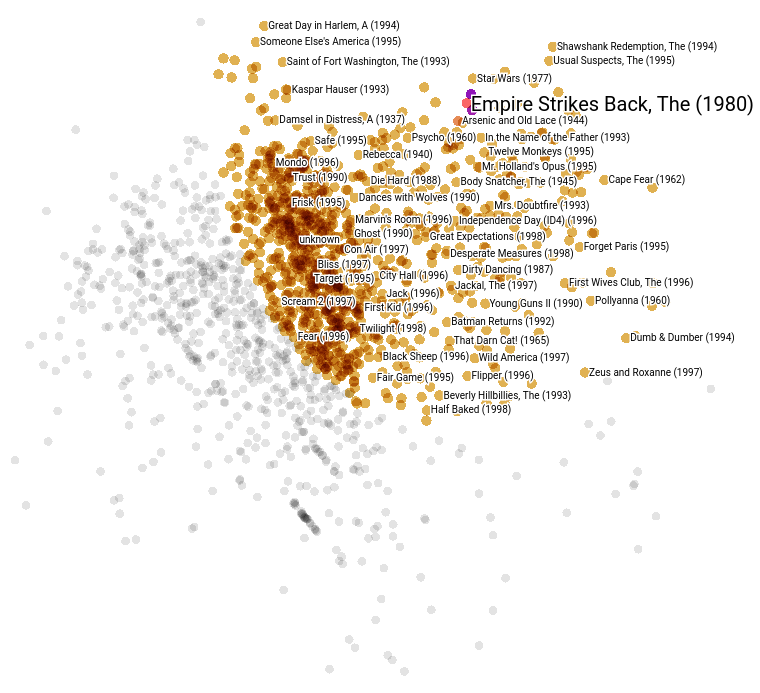
\includegraphics[width=0.49\textwidth]{movies}
	\caption{
		The embeddings of all movies in MovieLens100K dataset:
		The Empire Strikes Back is the reference movie, highlighted in red.
		The 1000 closest movies are highlighted in orange.
		A portion of movies have their titles displayed.
		This embedding shows the overall distribution of movies where similar movies such as Star Wars (1997) are closer to the reference movie.
	}
	\label{fig:movies}
\end{figure}

\subsection{Collaboration}
For this dataset, we select the country United States as the reference country and two other countries with similar economy, education and culture backgrounds as the two similar countries: United Kingdom and Germany.
Notice that we assume education and culture background have the most influence in international collaboration patterns.
The distances of a number of all countries to the reference country are shown in Table \ref{tab:countries-distance}.
\begin{table}[!ht]
	\centering
	\caption{
		The distances of countries to the reference country for Collaboration dataset.
	}
	\begin{tabular}{ccc} \hline \rowcolor{blue!30}
		Country & Distance & Similarity \\ \hline
		United States & 0 & self (reference) \\ \hline
		China & 0.216 & most similar \\ \hline
		... & ... & ... \\ \hline
		United Kingdom & 0.411 & more similar \\ \hline
		Germany & 0.483 & more similar \\ \hline
		... & ... & ... \\ \hline
		Jamaica & 29.531 & median point \\ \hline
		... & ... & ... \\ \hline
		Senegal & 31.018 & less similar \\ \hline
		Peru & 31.259 & less similar \\ \hline
		... & ... & ... \\ \hline
		Zimbabwe & 32.283 & least similar \\ \hline
	\end{tabular}
	\label{tab:countries-distance}
\end{table}
The data strongly suggest that the distances from similar countries to the reference country are much shorter than that from the median point.
The embeddings of all countries are shown in Figure \ref{fig:countries}.

\begin{figure}[!ht]\centering
	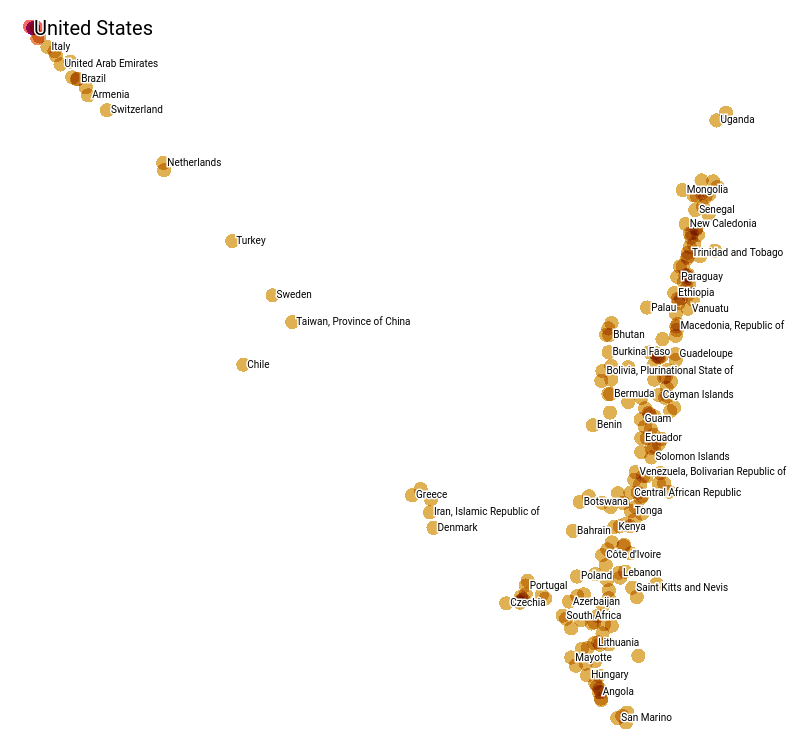
\includegraphics[width=0.49\textwidth]{countries}
	\caption{
		The embeddings of countries in Collaboration dataset:
		The United States is the reference country, highlighted in red.
		A portion of the countries have their names displayed.
		This embedding shows the overall distribution of countries where similar countries such as Italy are closer to the reference country.
	}
	\label{fig:countries}
\end{figure}

\section{Conclusions}
These experiment results support our hypothesis that the knowledge Model R learns is indeed meaningful node embeddings where similar nodes (based on their semantics associated with the specific domain) are close to each other in the node embedding space.
Moreover, these results provide strong evidences for the claim in the original Model R paper that Model R learns knowledge of nodes (in the form of node embeddings) from the known link weights and uses that knowledge to predict unknown link weights.
On a broader scope of deep learning application domains, this paper provides direct evidences that deep learning based embedding techniques are effective through embedding analyses and visualizations for two other application domains after natural language processing: recommender systems and graph mining.

\section{Future work}
The most important aspect we should work on in the future about this work is the metrics of node embedding.
As embeddings are ubiquitous and valuable in deep learning and the popularity of deep learning is on the rise, we believe an important question is: what are good embeddings?
A direct and naive answer can be: embeddings that match humans' perceptions of the nodes are good embeddings.
But humans' perceptions are, by nature, very complicated and subjective.
A few possible desirable metrics of good embeddings are discussed below.

\subsection{Similarity measurement}
Similar nodes should have their embeddings close to each other.
This is an obvious metric and also the one we tried to use intuitively for this work.
The distance measurement for embeddings is relatively easy but the similarity measurement for nodes is relatively hard.
One possible way to measure similarity is some type of statistics measurement of the behaviors of nodes.
For example, in recommender systems, it is natural to assume two users are very similar if they always give the same ratings to each of the movies.
But this is not easy to measure if there are few movies rated by both users.
Another possible way to measure similarity is some type of measurement of the distance of their attribute vectors.
For example, the attribute vector of a user can be [age, gender, occupation, location] as exposed by the metadata.
But it is hard to know what are the attributes most relevant to users' movie preferences.

\subsection{Relation measurement}
Node pairs with the same logical relation should have their embeddings with same spacial relation.
This one is less obvious and the logical relation measurement for nodes is hard.
In natural language processing, words can have very clear logical relations such as (male, female) relation in word pairs including [(gentleman, lady), (king, queen), (father, mother), (uncle, aunt)].
We have not identified any way to measure the logical relations for nodes.
For example, it is rather difficult to define any logical relation for two users or countries.

\subsection{Prediction accuracy measurement}
Good embeddings should produce good prediction accuracy, despite the type of node targeted for prediction.
This one is very obvious because eventually some other machine learning system is to use these embeddings to do predictions.
Therefore, good metrics should have positive correlation with prediction accuracy of the later stages of the deep learning system whose inputs are the embeddings.
This does not require any work with respect to the actual nodes but it is still hard to measure: some embeddings might work well on some models but not on other models so it is hard to decide which model should be used as the evaluation reference.

\section*{Acknowledgements}
This material is based upon work supported by Grant No. number.

\bibliographystyle{IEEEtran}
\bibliography{references}
\end{document}
